\chapter{Test}\label{Test}
\setcounter{secnumdepth}{5}

\begin{longtabu} to \linewidth{@{}l l l X[j]@{}}
    Version &    Dato &    Ansvarlig &    Beskrivelse\\[-1ex]
    \midrule
    0.1 &	8/09 2015	&	Alle		& Oprettelse  af dokument\\
    0.2 &	09/12 2015 	& SSK, NHL, FRM & Påbegyndelse af hardware testafsnit\\
    0.3 &	09/12 2015 	& TSN, JTH, MFJ & Påbegyndelse af software testsafsnit \\
    1.0 & 15/12 2015	& Alle & Rettelser\\
\label{version test}
\end{longtabu}

\section{Indledning} 
Testafsnittet giver en beskrivelse af hvilke tests, der løbende er blevet foretaget på både hardware og software. Testene består af modultest, hvor enkelte delelementer af systemet testes uafhængigt af hinanden. Modultesten er til for at verificere de enkelte enheder virker efter hensigten.\\
En mere omfattende test, i form af en integrationstest, hvor de større dele af både hardware og software testes afhængigt af hinanden. Ved integrationstesten ligger fokus på, hvordan systemet fungerer, set fra udviklers synspunkt.\\ 
Begge tests ligger til grund for den endelige accepttest, hvor testen ses fra kundens synspunkt.

\section{Modultest hardware}\label{ModulHard}

Til test af hardwaredelen blev der først udført modultest på henholdsvis forstærkeren og det analoge filter. Efterfølgende blev der udført integrationstest på forstærkeren og det analoge filter sat sammen med tryktransduceren. Slutteligt blev den samlede hardwaredel bestående af tryktransducer, forstærker og analogt filter testet på en vandsøjle.\\
Resultater kan ses i bilag \ref{Modul og integration}.

\subsection{Modul test af forstærkeren}
I modultesten af forstærkeren blev Analog Discovery brugt som spændingsforsyning, signalgenerator og oscilloskop på to forskellige målepunkter placeret ved henholdsvis indgangssignalet og udgangssignalet.\\
Da tryktransduceren forventes at have output-spændinger i området 0 til 6,25mV blev signalet fra transduceren simuleret ved en sinus på 1Hz uden offset. Den laveste amplitude for indgangssignalet var 1mV. For hver måling blev amplituden for indgangs signalet sat op med 1mV indtil den sidste måling, hvor amplituden var nået op på 10 mV. Således blev der 10 forskellige målinger. Reelt set var det kun nødvendigt at teste op til 6mV eller 7mV, da det er herimellem, at man kan forvente et max tryk fra transduceren vil ligge. Da der alligevel er taget målepunkter op til 10mV, skyldes det, at der ved flere målinger kan laves en ”pænere” tendenslinje ved lineær regression. Opstillingen til denne test ses på figur \ref{fig:ForstaerkerTest}:

\begin{figure}[H]
	\centering
	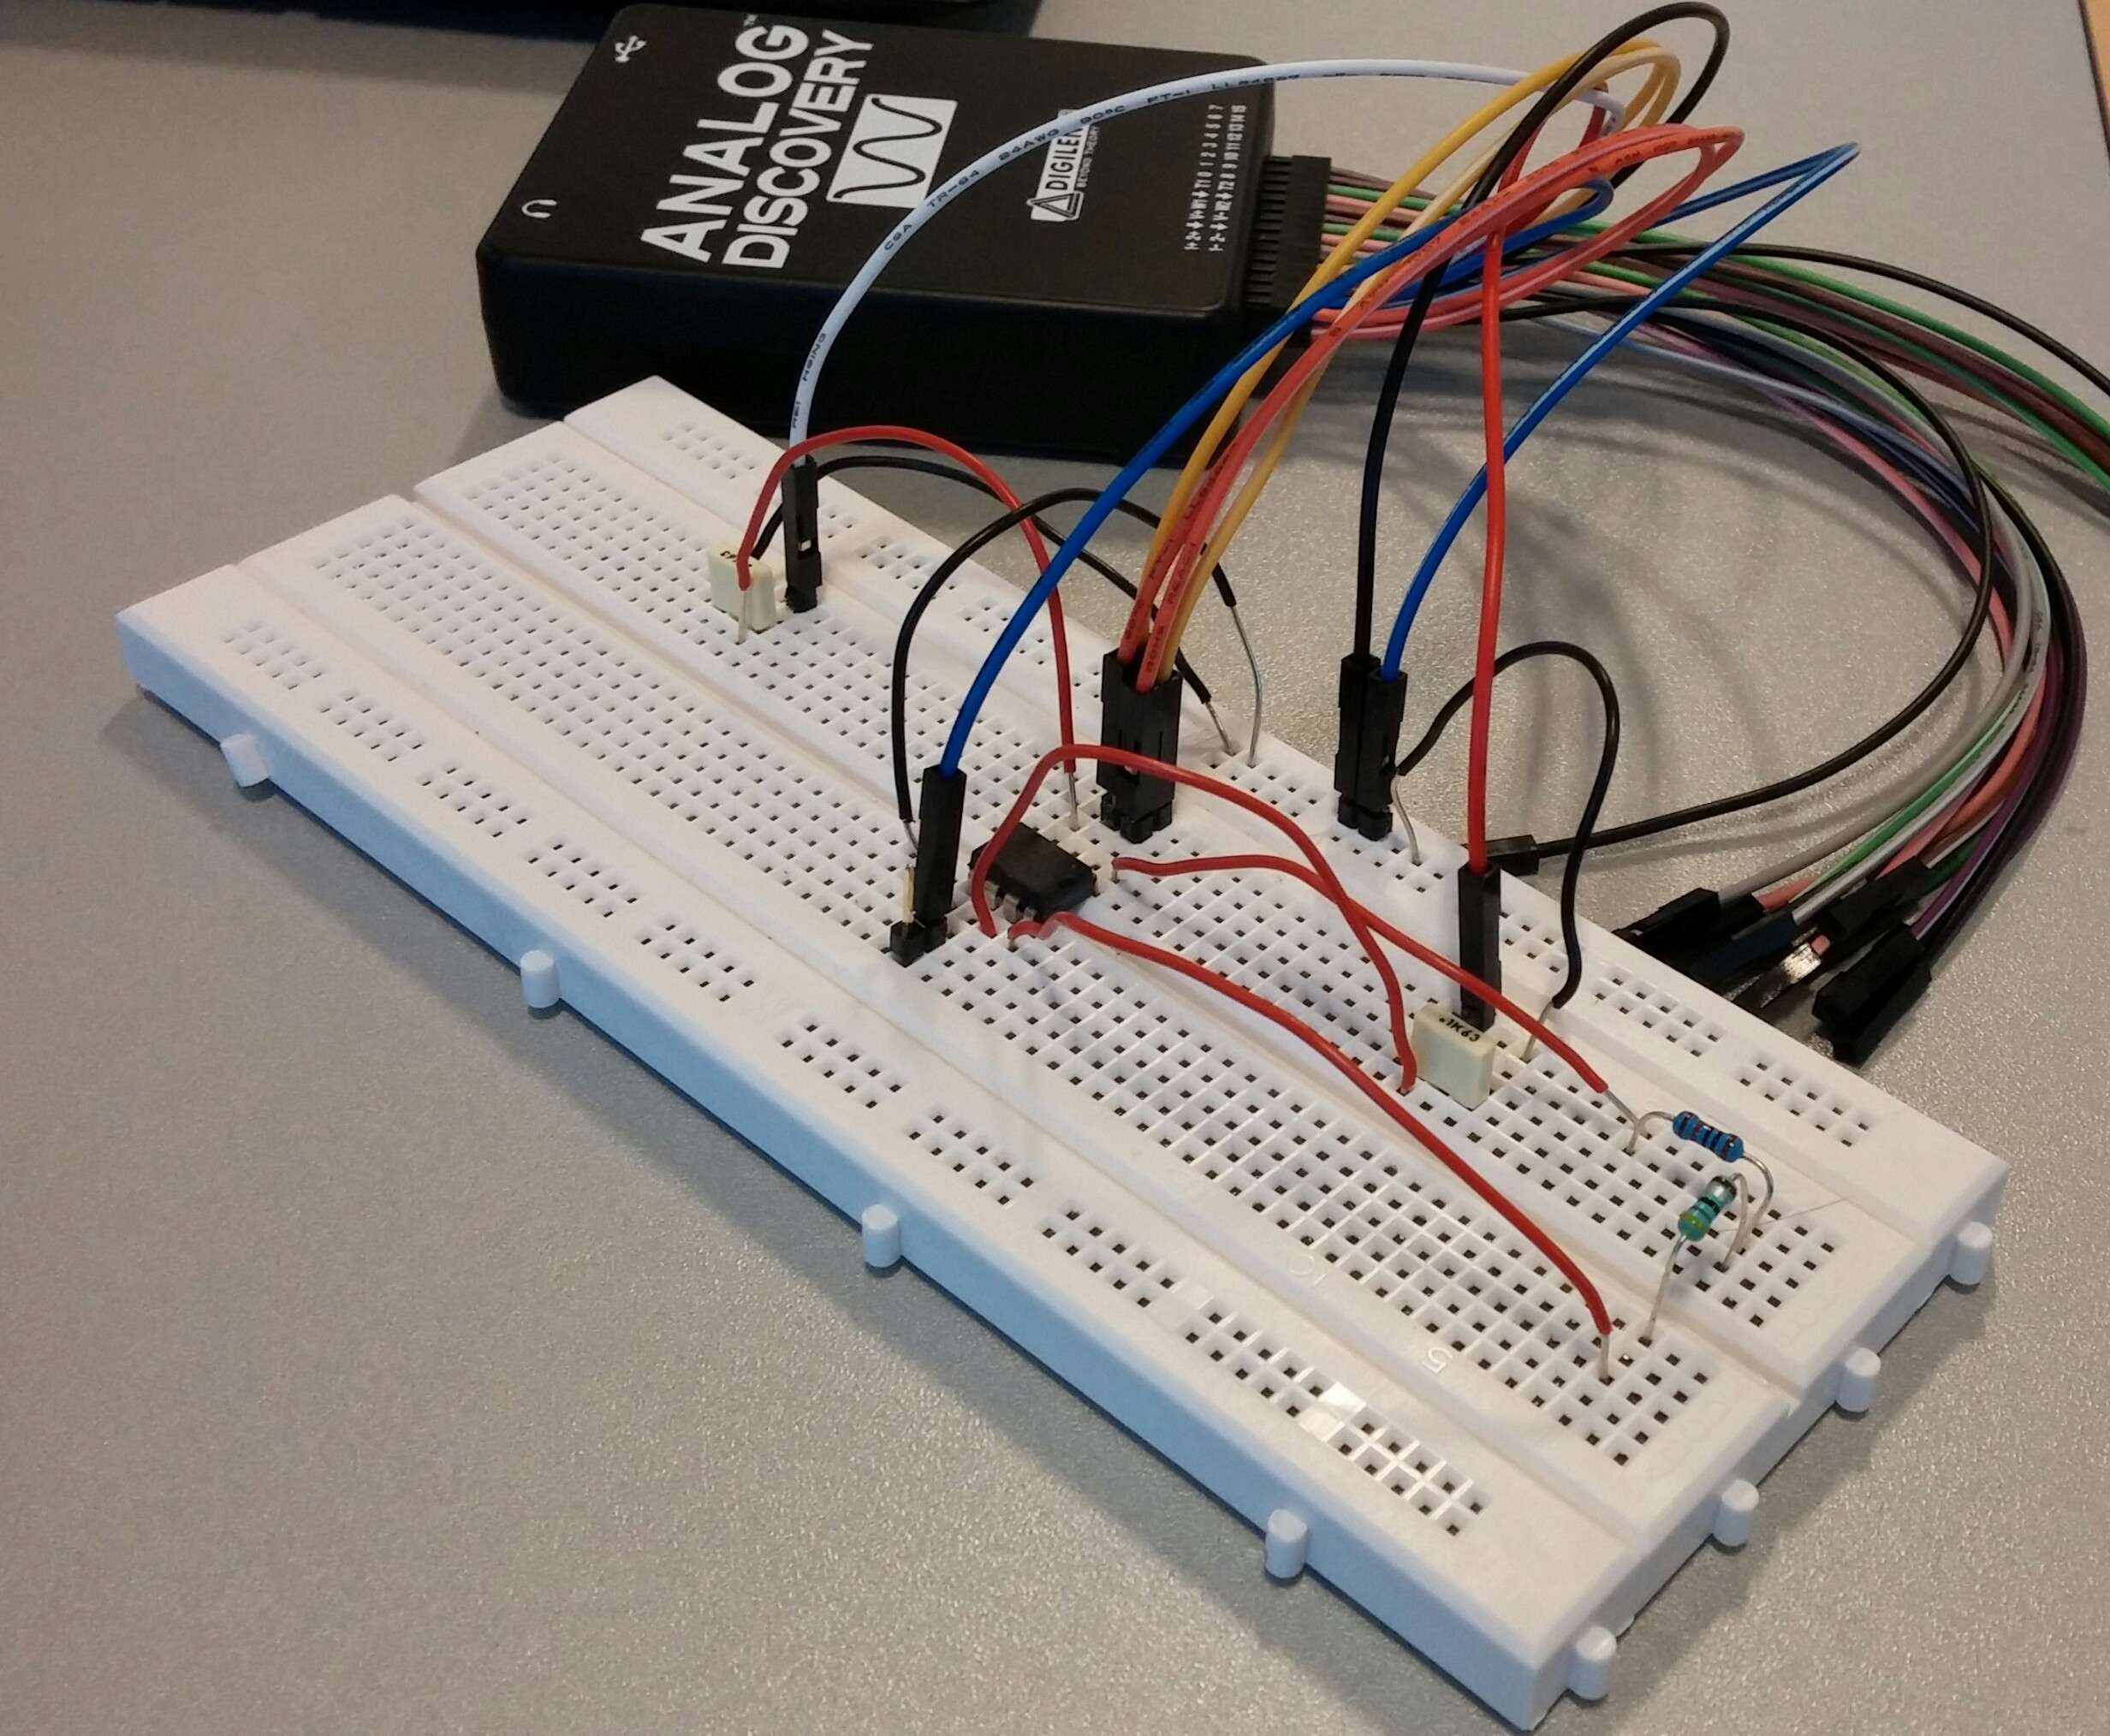
\includegraphics[width=0.7\textwidth]{Figurer/Hardware/ForstaerkerTest}
	\caption{Måleopstilling ved modul test af forstærkeren.}
	\label{fig:ForstaerkerTest}
\end{figure}

Ud af målingerne blev der foretaget lineær regression over de 10 målepunkter. Tendenslinjen der kom ud af den lineære regression blev som vist på figur \ref{fig:SinusModul}:

\begin{figure}[H]
	\centering
	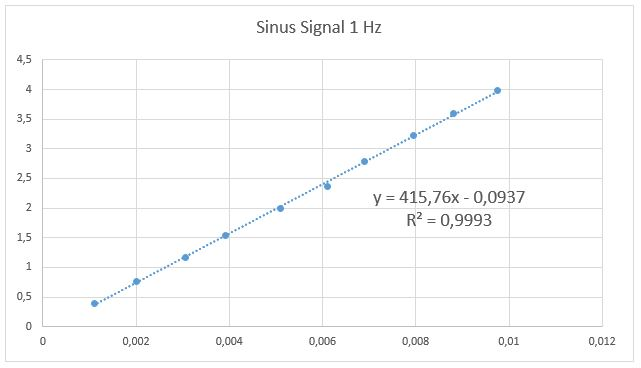
\includegraphics[width=0.7\textwidth]{Figurer/Hardware/Sinusforstaerker}
	\caption{Målpunkter samt tendenslinje for målingerne ved modultest af forstærkeren med 1Hz sinus-signal.}
	\label{fig:SinusModul}
\end{figure}


I figur \ref{fig:SinusModul} kan Y beskrives som værende forstærkningen ved en given frekvens. Konstanten 415,8 er den reelle forstærkning som er målt for forstærkeren. Skæringen med y-aksen burde være 0, men grundet måleusikkerheder er den blevet -0,09, hvilket også er acceptabelt. Den høje R$^2$ værdi indikerer, at der er en tydelig lineær sammenhæng mellem den påtrykte spænding og spændingen af output, dvs. forstærkningen er lineær.\\[1ex]
Senere påtryktes samme måleopstilling et DC-signal med amplituder startende fra 3mV op til 10mV. Igen blev amplituden øget med 1mV for hvert måling således, at der blev 7 målepunkter. Ved målinger foretaget på signaler med både 1mV og 2mV er offsettet i Analog Discovery så stort, at målingerne ikke kan foretages.

Forstærkning, som blev beregnet på baggrund af de målte output og input, viste sig at være meget varierende. Der blev beregnet forstærkninger fra et sted mellem 455 gange og 784 ganges forstærkning. Jo lavere offset desto større forstærkning. Ud fra denne iagttagelse blev det antaget, at denne meget store afvigelse måtte skyldes et negativt offset i Analog Discovery. 
\\For at finde frem til dette offset blev output-spændingen divideret med 400, som var den ventede forstærkning. Det målte input og resultatet fra den forrige udregning blev trukket fra hinanden. Heraf sås det, at offsettet for Analog Discovery måtte være 1,2mV.\\
Dette blev eftertestet med et digitalt multimeter, der rigtig nok målte 1,2mV højere på indgangen af forstærkeren end det som Analog Discovery målte. Opstillingen hertil ses i figur \ref{fig:DigitalMulti}:

\begin{figure}[H]
	\centering
	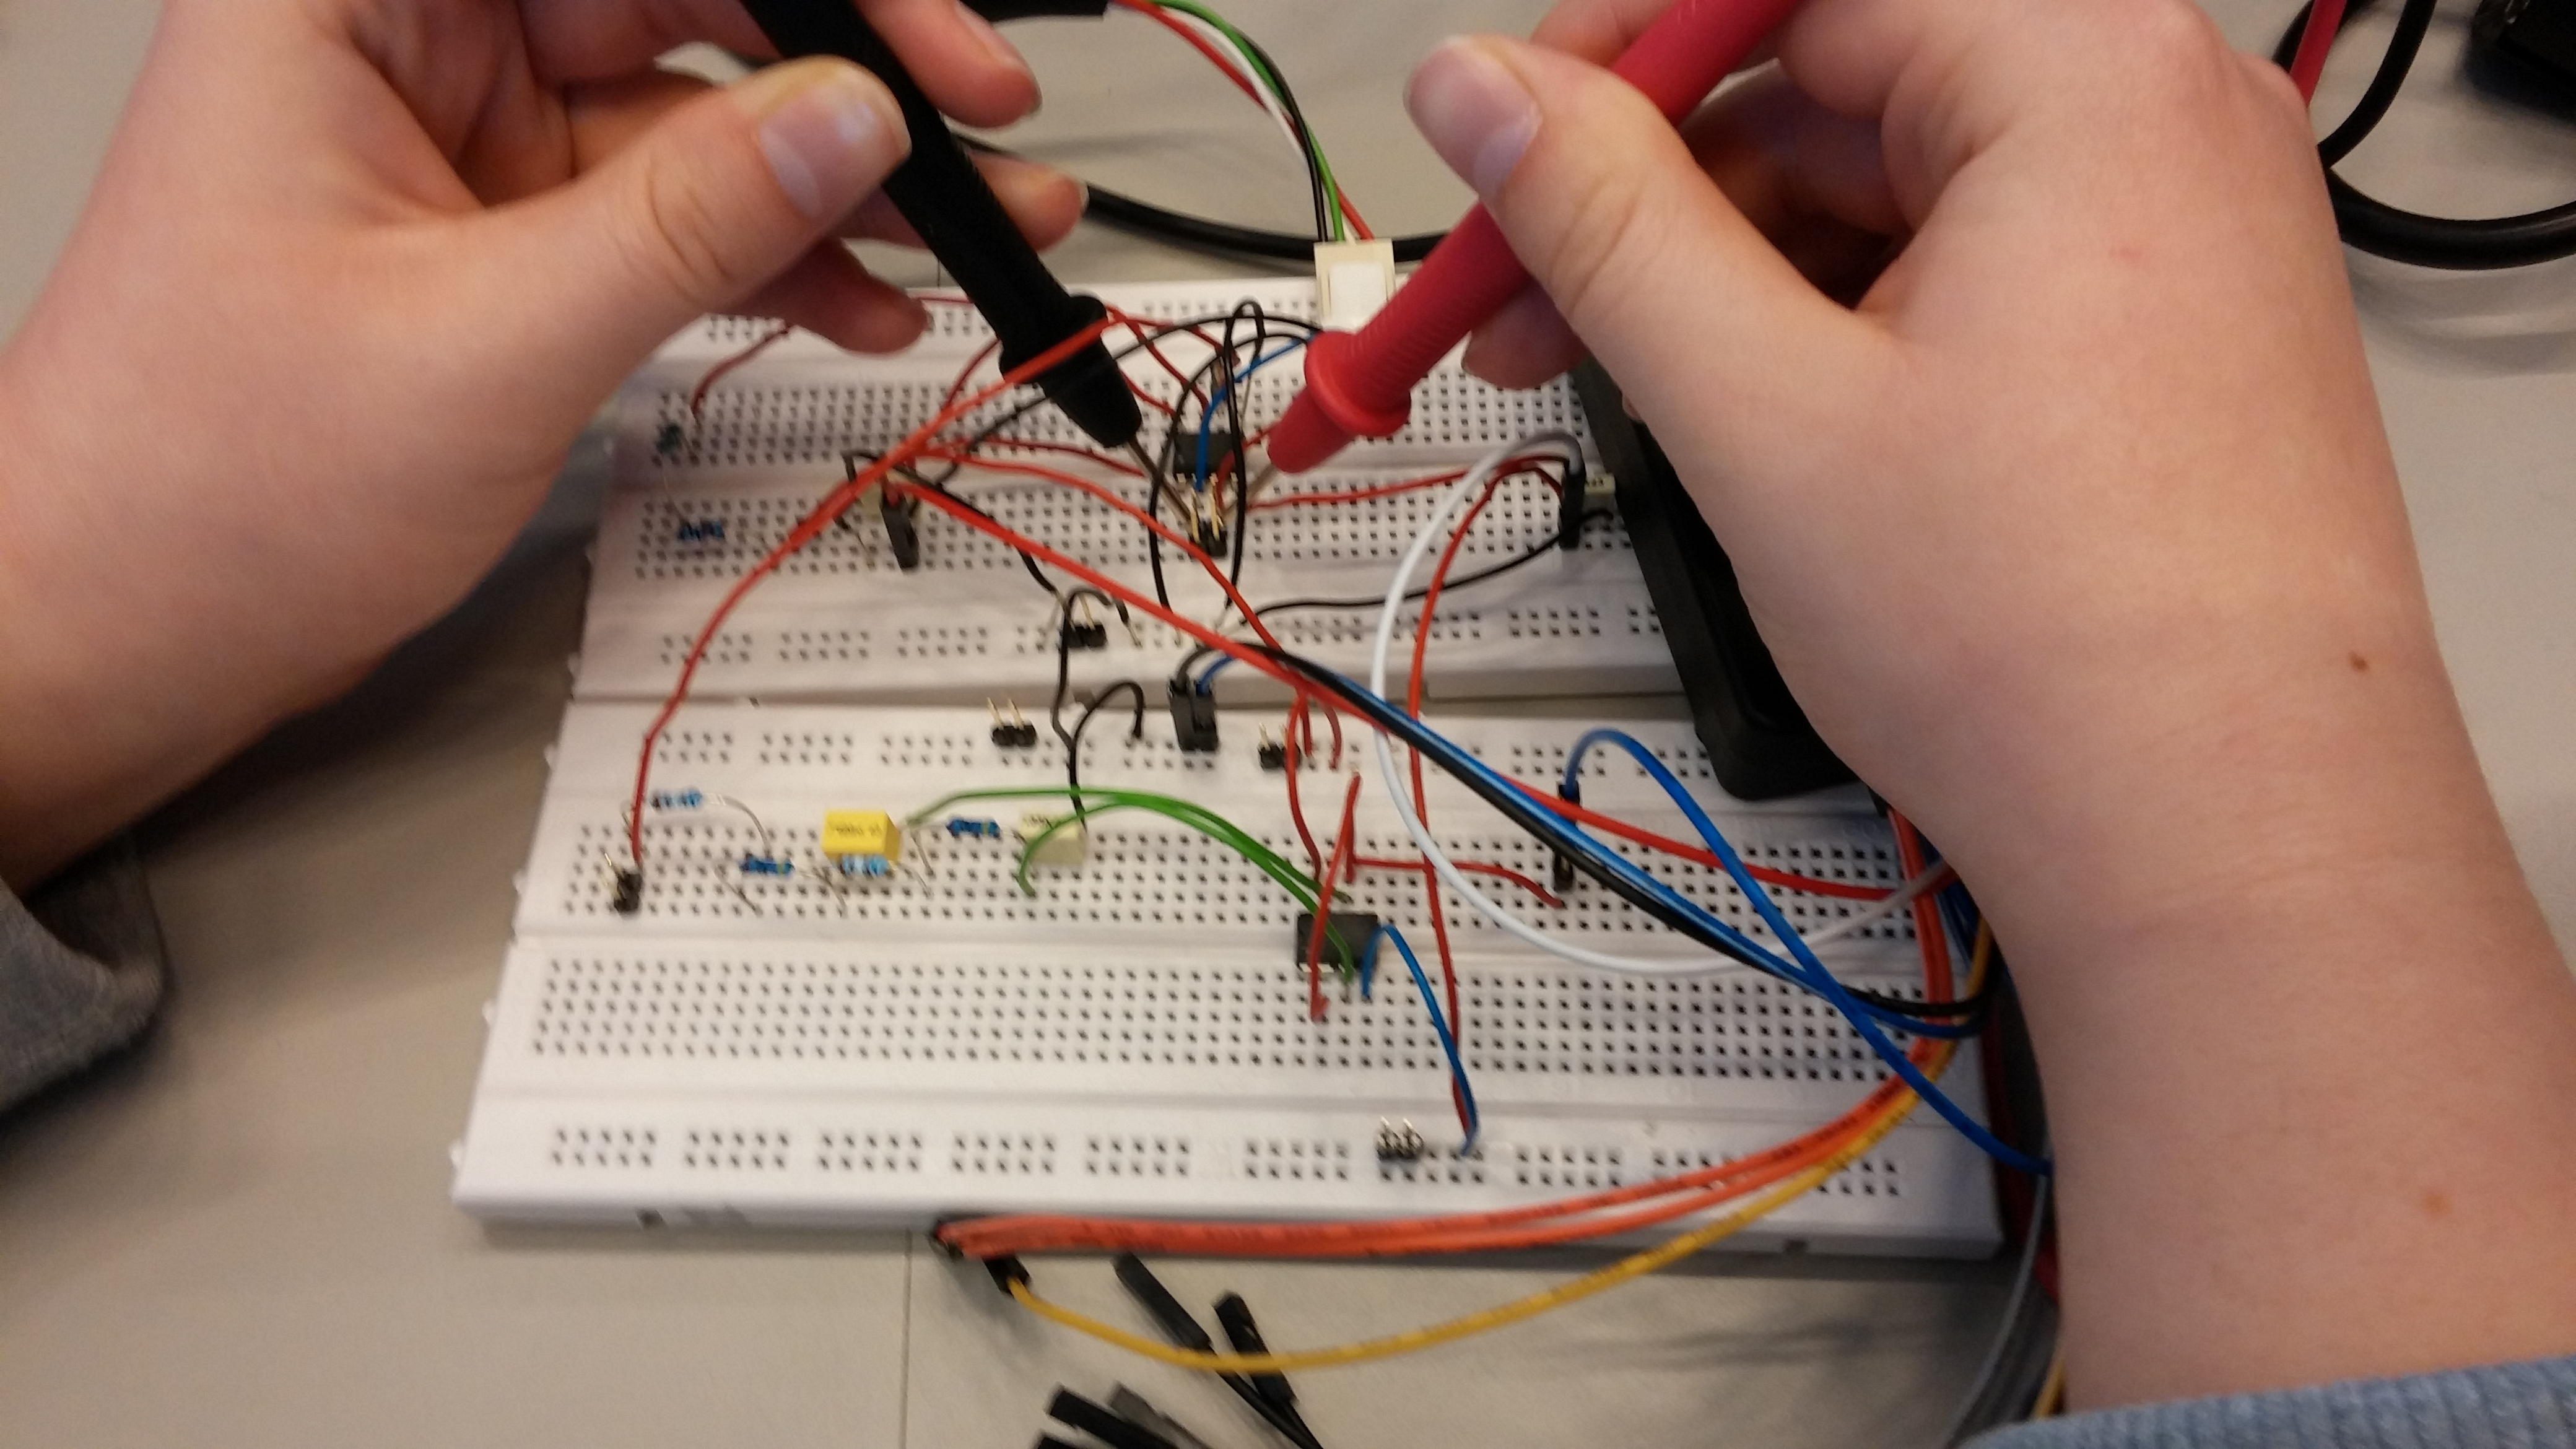
\includegraphics[width=0.7\textwidth]{Figurer/Hardware/DigitalMultimeter}
	\caption{Måling på indgangen af forstærkeren med det digitale multimeter.}
	\label{fig:DigitalMulti}
\end{figure}

Efter at have foretaget lineær regression på de syv målepunkter så tendenslinjen ud som følger på figur \ref{fig:DCModul}:

\begin{figure}[H]
	\centering
	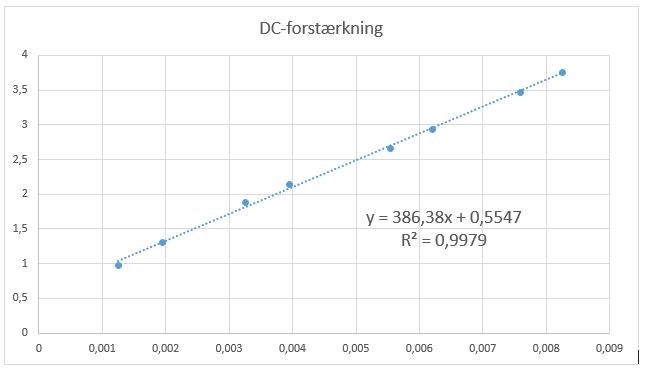
\includegraphics[width=1\textwidth]{Figurer/Hardware/DCforstaerkning}
	\caption{Målpunkter samt tendenslinje for målingerne ved modultest af forstærkeren med DC-signal.}
	\label{fig:DCModul}
\end{figure}

Ud af figur \ref{fig:DCModul} ses, at forstærkningen givet ud fra de syv målepunkter er på 386, hvilket er en del under den målte forstærkning, når systemet påtrykkes et sinussignal i stedet for et DC-signal. Dette kan skyldes, at der i målingen af DC-signalet er færre målepunkter, og at det dermed bliver en mere usikker måling, da selv en mindre måleusikkerhed har en større indflydelse på den målte forstærkning.

\subsection{Modul test af det analoge filter}
I modultesten af det analoge filter blev Analog Discovery brugt som spændingsforsyning, signalgenerator og som oscilloskop til at måle amplituderne for input-signalet og output-signalet for filteret. Måleopstillingen hertil ses på figur \ref{fig:FilterTest}:

\begin{figure}[H]
	\centering
	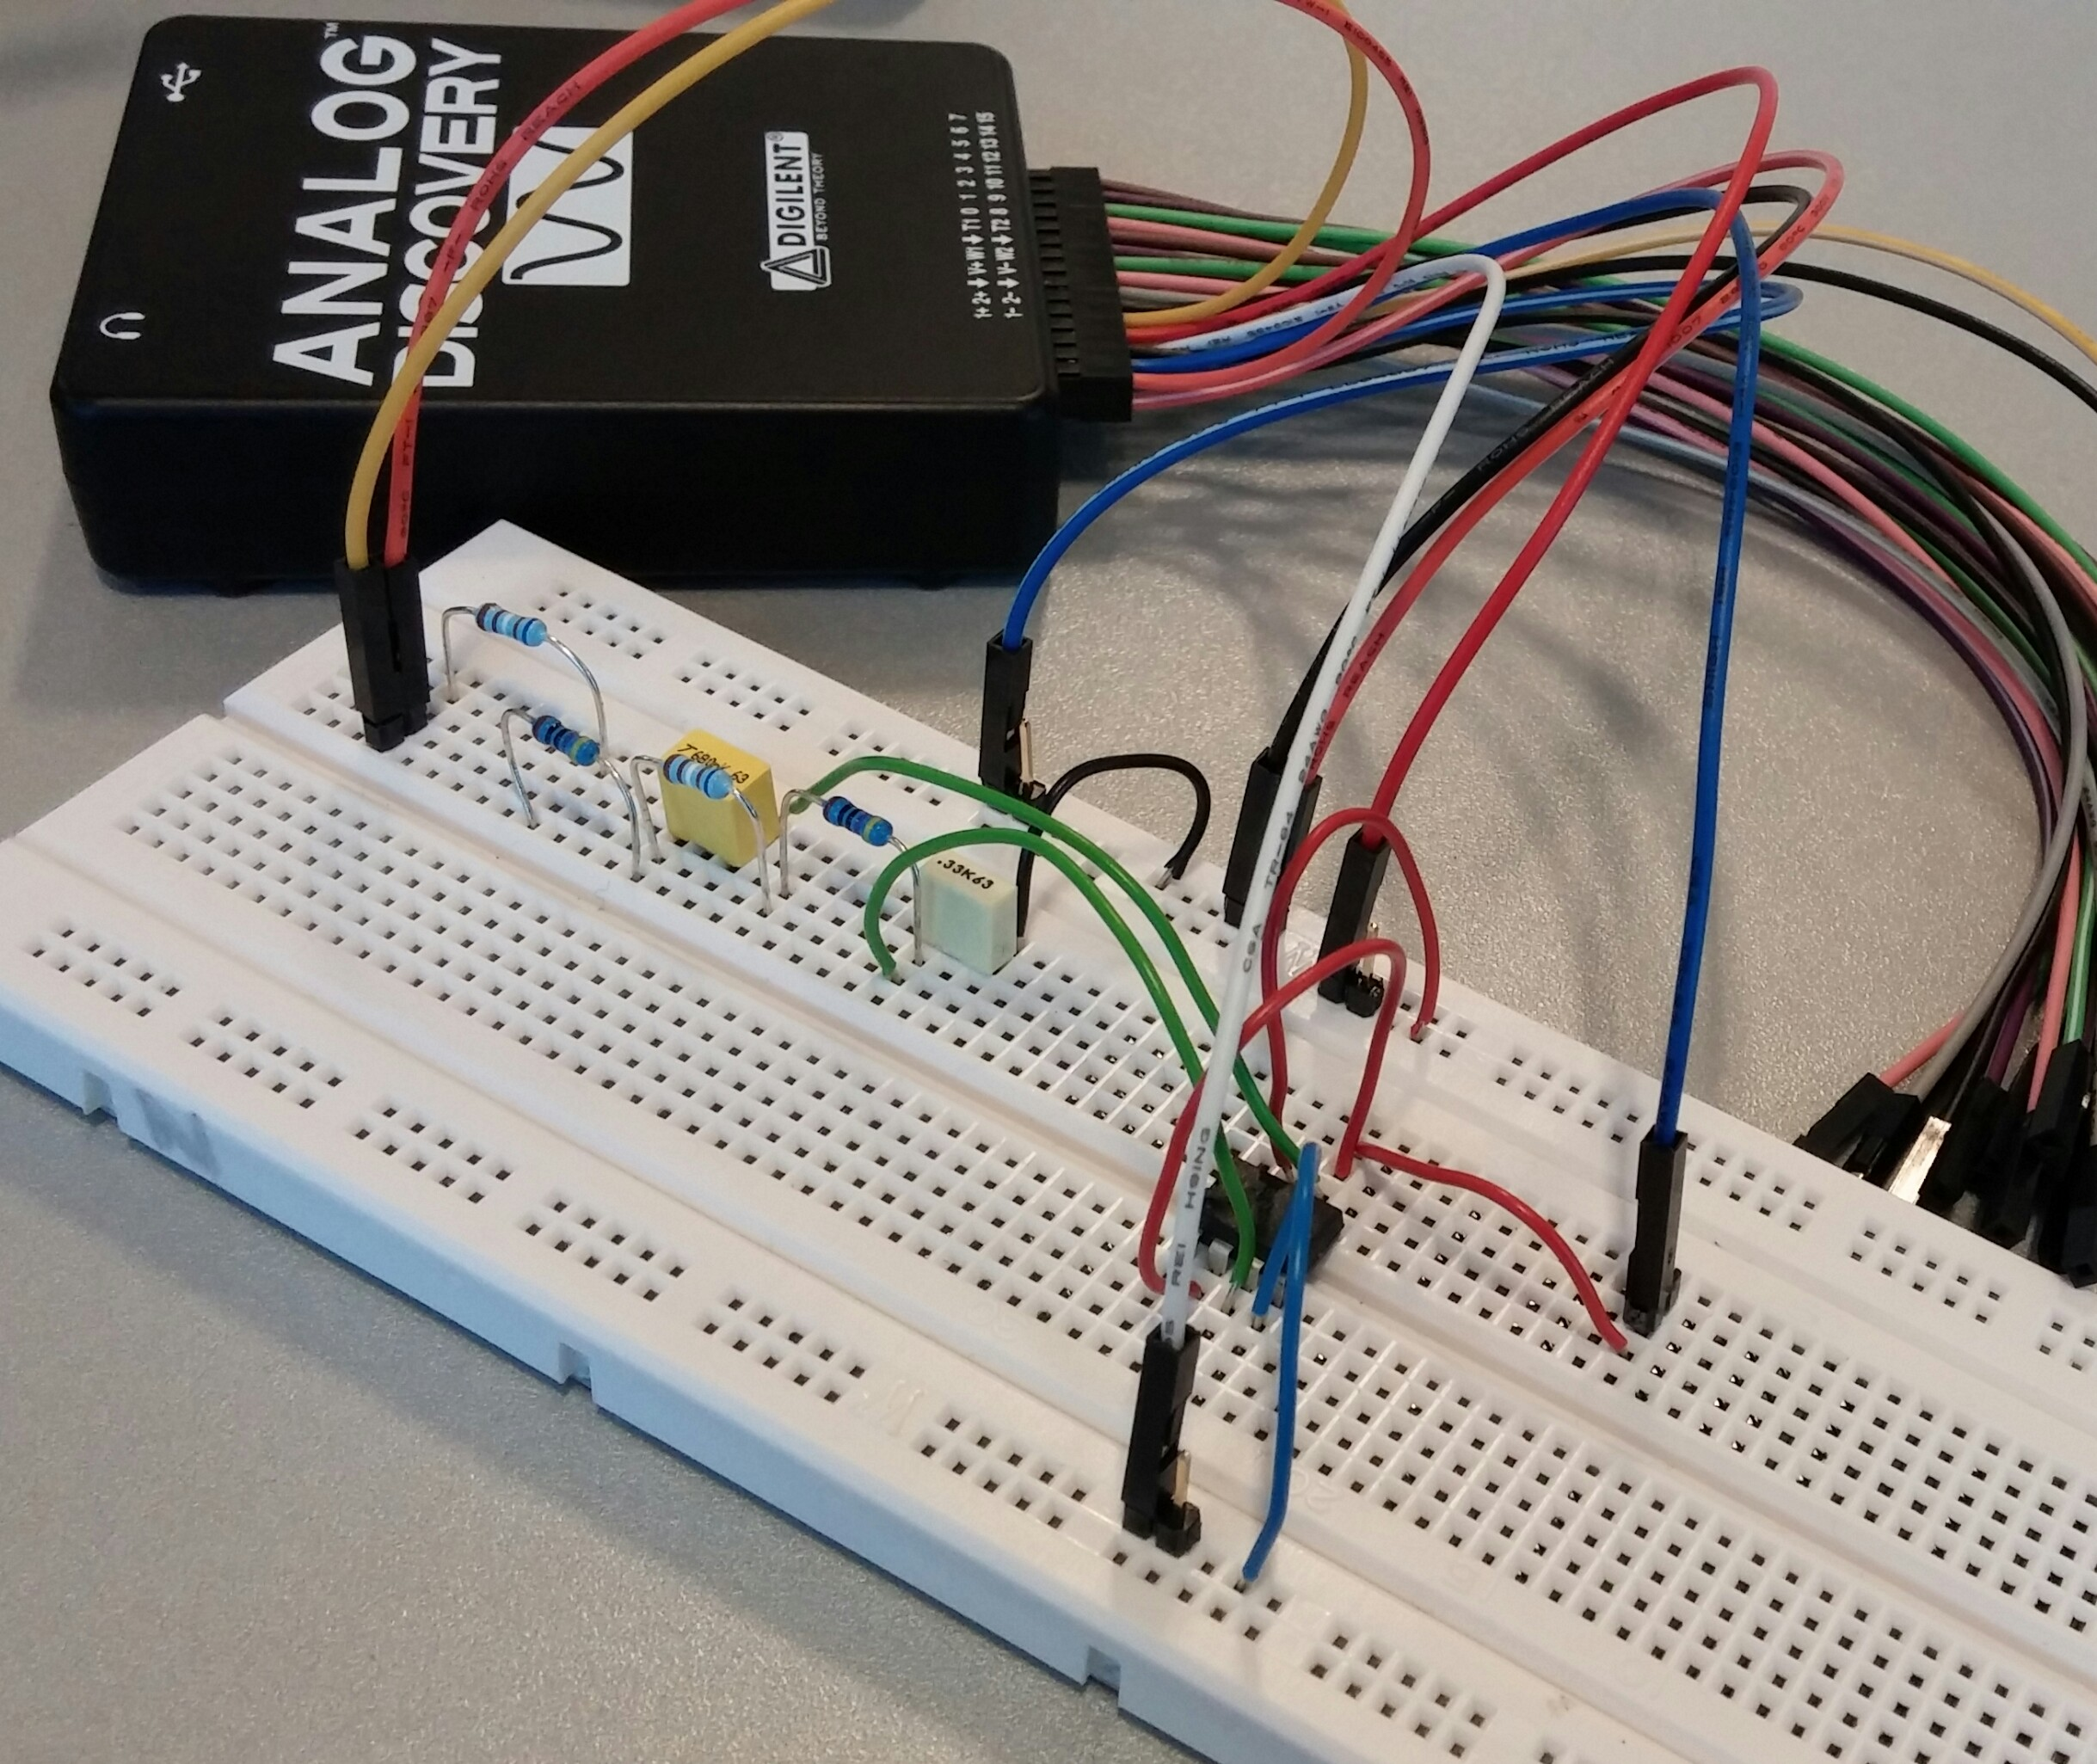
\includegraphics[width=0.5\textwidth]{Figurer/Hardware/FilterTest}
	\caption{Måleopstilling ved modultest af det analoge filter.}
	\label{fig:FilterTest}
\end{figure}

I modultesten af det analoge filter ændres frekvensen for det påtrykte sinussignal på filter indgangen. Der blev målt på i alt 21 målepunkter som lå i intervallet 1Hz til 500Hz; se bilag \ref{Modul og integration} for de præcise angivelser af de udvalgte målefrekvenser. Output-amplituden samt $\Delta$t mellem de to grafer blev aflæst. På baggrund af disse målinger blev dæmpningen af signalet afbildet, hvilket ses på figur \ref{fig:FilterAmplitude}. 

\begin{figure}[H]
	\centering
	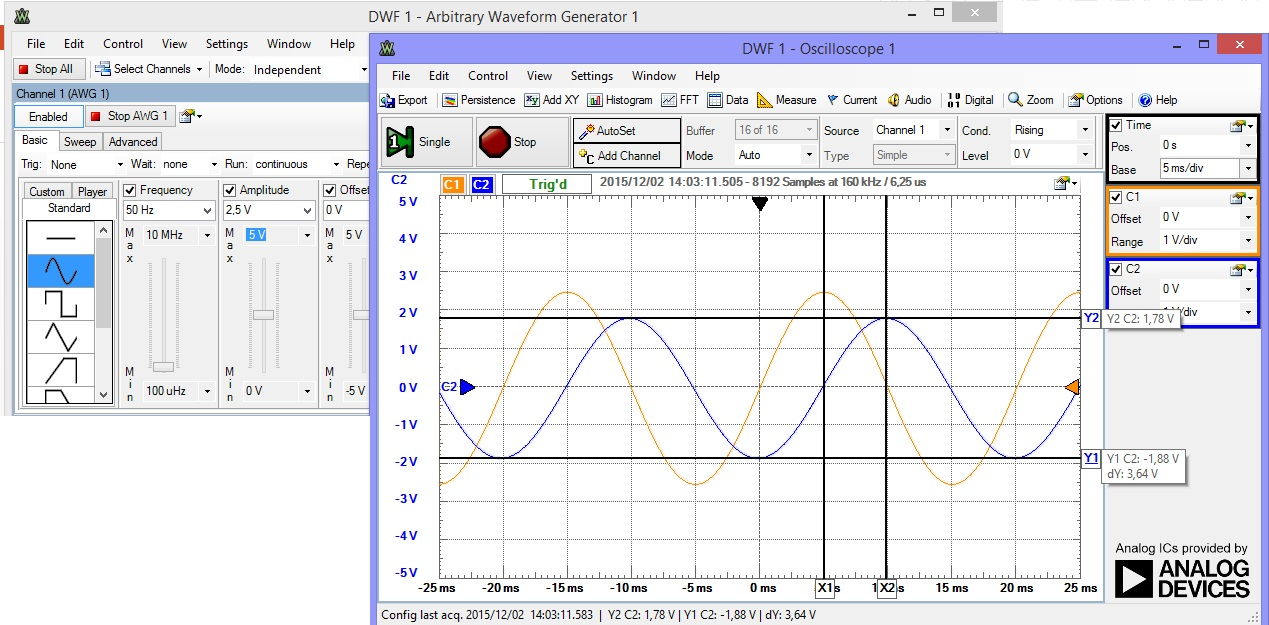
\includegraphics[width=1\textwidth]{Figurer/Hardware/AnalogScreenFilterAmp}
	\caption{Aflæsning af amplitude størrelse for outputsignalet, C2, fra filteret når inputsignalet, C1, har en amplitude på 2,5V}
	\label{fig:FilterAmplitude}
\end{figure}

Ved brug af 3dB frekvensen er det muligt at vurdere om knækfrekvensen for filteret er som den skal være. Denne kan udregnes ved følgende ligning \ref{ligning3db}:

\begin{align}
3dB_{frekvens}=\frac{V_{max}}{\sqrt{2}}
\label{ligning3db}
\end{align}
I dette tilfælde bliver udregningen som vist i ligning \ref{ligning3db4}:\\
\begin{align}
	3dB_{frekvens}=\frac{2,5V}{\sqrt{2}}=1,76V
	\label{ligning3db4}
\end{align}
Ved omregning af de 1,76V til dB fås 4,9dB. Hvis filteret virker efter hensigten skal frekvensen ved 4,9dB være 50Hz. Denne kan aflæses i figur \ref{fig:AmplitudedBFilter}

\begin{figure}[H]
	\centering
	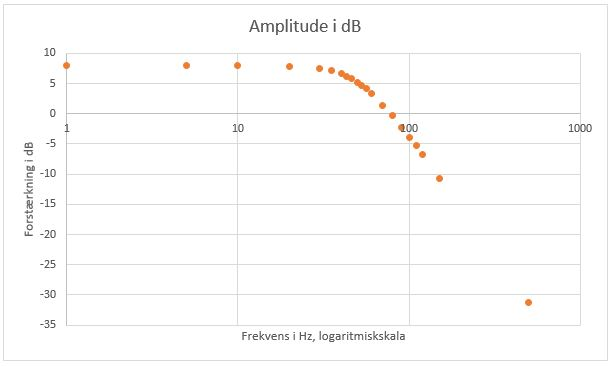
\includegraphics[width=1\textwidth]{Figurer/Hardware/AmpdBFilter}
	\caption{Forstærkningen i dB set i forhold til den frekevens som det påtrykte signal har.}
	\label{fig:AmplitudedBFilter}
\end{figure}

Som det kan ses ud af figur \ref{fig:AmplitudedBFilter} er forstærkningen ved 3dB frekvensen et sted imellem de to målepunkter på 50Hz og 53Hz. Derfor må filterets knækfrekvens ligge mellem 50Hz og 53Hz.

Herefter blev tidsforskydningen aflæst, således at fasedrejet kunne udregnes. Faseforskydningen ved de forskellige frekvenser er vist på figur \ref{fig:FilterTidsforskydning}:

\begin{figure}[H]
	\centering
	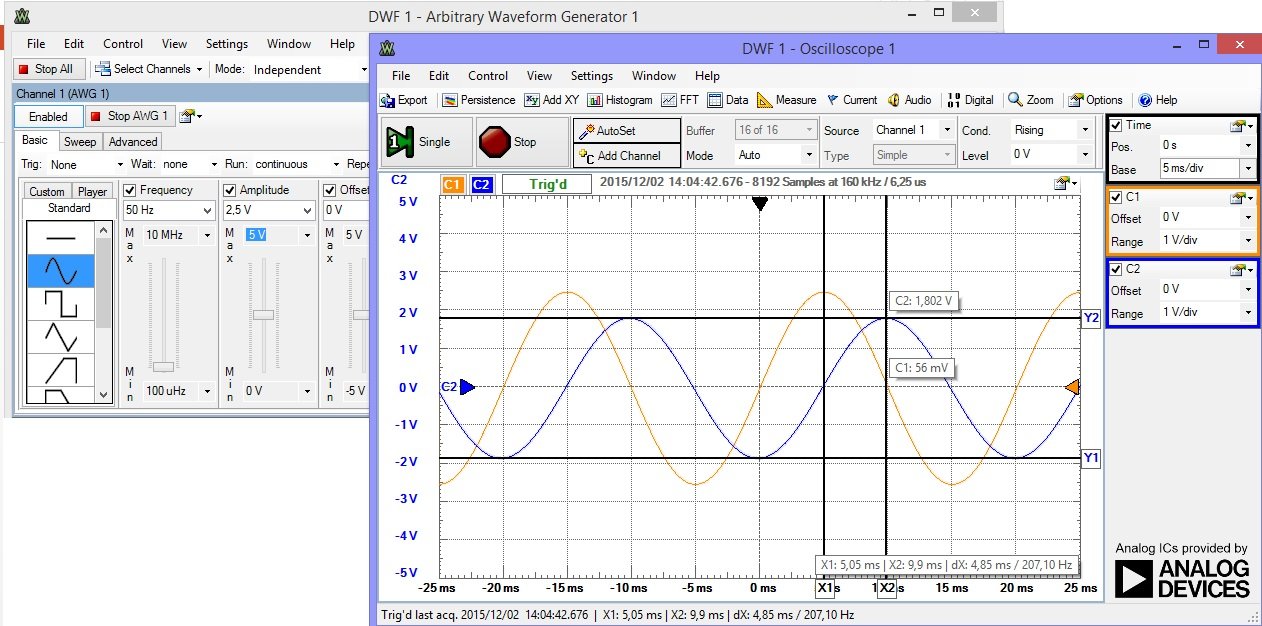
\includegraphics[width=1\textwidth]{Figurer/Hardware/AnalogScreenFilter}
	\caption{Aflæsning af tidsforskydningen for outputsignalet, C2, fra filteret set i forhold til indgangssignalet C1}
	\label{fig:FilterTidsforskydning}
\end{figure}

Det gælder generelt for et 2.ordens filter af standarttypen som der er arbejdet med igennem projektet, at fasen er 0$^{\circ}$ en dekade før filterets knækfrekvens og falder med 90$^{\circ}$/dekade frem til dekaden efter knækfrekvensen. Derfor skal filteret i praksis have et fasedrej på -90$^{\circ}$ ved knækfrekvensen 50Hz.\\ 
\begin{figure}[H]
	\centering
	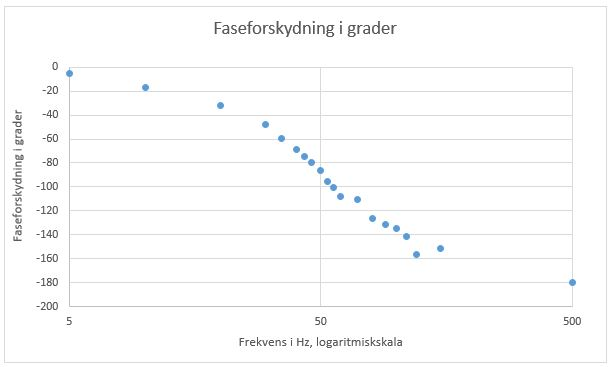
\includegraphics[width=1\textwidth]{Figurer/Hardware/FaseforskydningFilter}
	\caption{Faseforskysningen målt ved forskellige frekvenser for det analoge filter.}
	\label{fig:FilterFaseforskydning}
\end{figure}

Som det ses ud af figur \ref{fig:FilterFaseforskydning} er fasedrejet ved frekvensen 5Hz på -5,2$^{\circ}$, denne skulle reelt set have været 0$^{\circ}$. \\
Ved knækfrekvensen som er sat til 50Hz er fasedrejet -86,4$^{\circ}$, hvor fasedrejet skulle have været -90$^{\circ}$. Ved målingen for 53Hz er fasedrejet -95,4$^{\circ}$. Dermed kan der argumenteres for, at filterets reelle knækfrekvens må ligge et sted imellem 50Hz og 53Hz. 
For målingen på 500Hz er fasedrejet -180$^{\circ}$, hvilket stemmer overens med teorien for 2.ordens filterets fasekarakteristik.

\section{Integrationstest hardware}

\subsection{Integrationstest for forstærker og analogt filter}
Til integrationstesten af forstærkeren og det analoge filter blev Analog Discoverys signalgenerator koblet til indgangen på forstærkeren, som blev påtrykt et sinussignal. Filter og forstærker blev koblet sammen således output fra forstærkeren løb over i filterets input. Analog Discovery blev brugt som oscilloskop på det analoge filters udgang. Desuden fungerede Analog Discovery som spændingsforsyning for både forstærkeren og det analoge filter.\\
Der blev udført to målinger for hver udvalgte målefrekvens, hvor amplituden af sinussignalet var henholdsvis 6mV og 7mV. Der blev dermed foretaget to målinger for hver af de 16 frekvenser, der lå i intervallet 1Hz til 1kHz, som ses i bilag \ref{Modul og integration}. Opstillingen ses på figur \ref{fig:ForstaerkerFilterOpstiling}:

\begin{figure}[H]
	\centering
	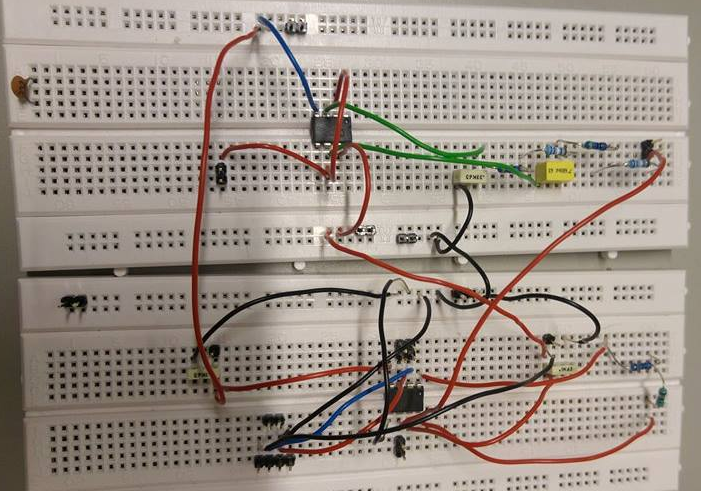
\includegraphics[width=0.7\textwidth]{Figurer/Hardware/samletopstilling}
	\caption{Opstillingen der blev brugt til test af forstærker og analogt filter}
	\label{fig:ForstaerkerFilterOpstiling}
\end{figure}

Da projektet tager udgangspunkt i, at et maksimalt blodtryk vil have en amplitude på 6,25mV, er de to måle amplituder 6mV og 7mV blevet udvalgt for på den måde at kunne eftervise, at forstærkeren og filteret sammen får forstærket signalet op som det skal. Samtidig er de forskellige målefrekvenser udvalgt med henblik på at vise, at signalet, på trods af forskellige indgangsamplitude, har den samme knækfrekvens, hvilket man kan se ud af figur \ref{fig:ForstaerkerFilterGraf}.

\begin{figure}[H]
	\centering
	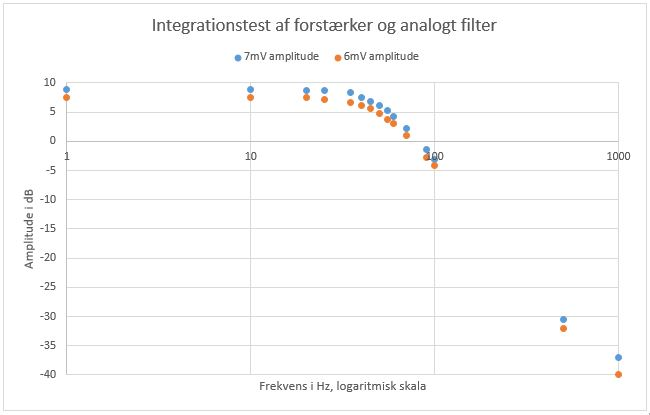
\includegraphics[width=0.7\textwidth]{Figurer/Hardware/IntegrationstestForstaerkerFilter2}
	\caption{Integrationstest resultater ved test af forstærker og analogt filter}
	\label{fig:ForstaerkerFilterGraf}
\end{figure}

Som det kan ses ud af \ref{fig:ForstaerkerFilterGraf} viser amplitudekarakteristikken for signaler ved hver af de to forskellige amplituder bliver forstærket relativt lige meget dvs. de to amplitudekarakteristikker følges ad.
Knækfrekvensen som med de pågældende komponentværdier er udregnet til værende 50,37Hz, se afsnit \ref{Implementering}. Knækfrekvensen kan findes på grafen ved at aflæse 3dB frekvensen.

For signalet med amplitudekarakteristikken for 7mV bliver 3dB frekvensen dermed som følger i ligning \ref{ligning3db2}:\\
\begin{align}
	3dB_{frekvens}=\frac{7mV}{\sqrt{2}}=4,95mV
	\label{ligning3db2}
\end{align}


Ved aflæsning på grafen kan man ud for ca. 5mV se, at grafen på x-aksen kan aflæses til at ligge meget tæt på et målepunkt, der ligger i datasættet hedder (55Hz, 5,2dB), se bilag \ref{Modul og integration}. Ud fra denne oplysning må det antages at den målte knækfrekvens ligger lige en anelse under 55Hz. Dog er den målte knækfrekvens for systemet højere end 50Hz da forstærkningen ved målingen for 50Hz er ca. 6dB.\\
Ud af grafen og det dertilhørende datasæt kan det også læses at forstærkningen falder med næsten 40dB/dekade efter knækfrekvensen med en afvigelse på 3,4dB.

\begin{figure}[H]
	\centering
	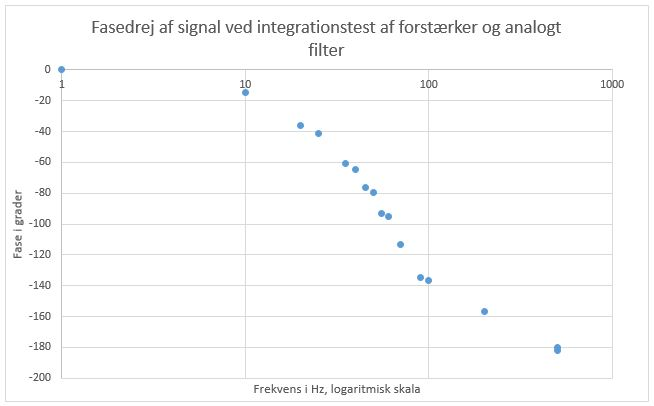
\includegraphics[width=0.7\textwidth]{Figurer/Hardware/FaseForstaerkerFilter}
	\caption{Fasedrej for signalet ved integrationstest af forstærker og analogt filter. Fasedrejningen af signalet er målt i grader i forhold til frekvens i Hz.}
	\label{fig:FaseForstaerkerFilter}
\end{figure}

Ud af \ref{fig:FaseForstaerkerFilter} ses det, at filteret og forstærkeren sammensat har et fasedrej på -90$^{\circ}$ ved et sted mellem 50Hz og 55Hz. Desuden ses det, at faseforskydningen allerede begynder en dekade før knækfrekvensen og er nede i -180$^{\circ}$ ved ca. en dekade over knækfrekvensen.

\subsection{Integrationstest med vandsøjle}
I integrationstesten med vandsøjlen blev hele hardwaredelen, dvs. transducer, forstærker og analogt filter, testet på en vandsøjle med et bestemt tryk. Transduceren blev koblet til vandsøjlen, som det ses af figur \ref{fig:IntegrationVandsoejle}: 

\begin{figure}[H]
	\centering
	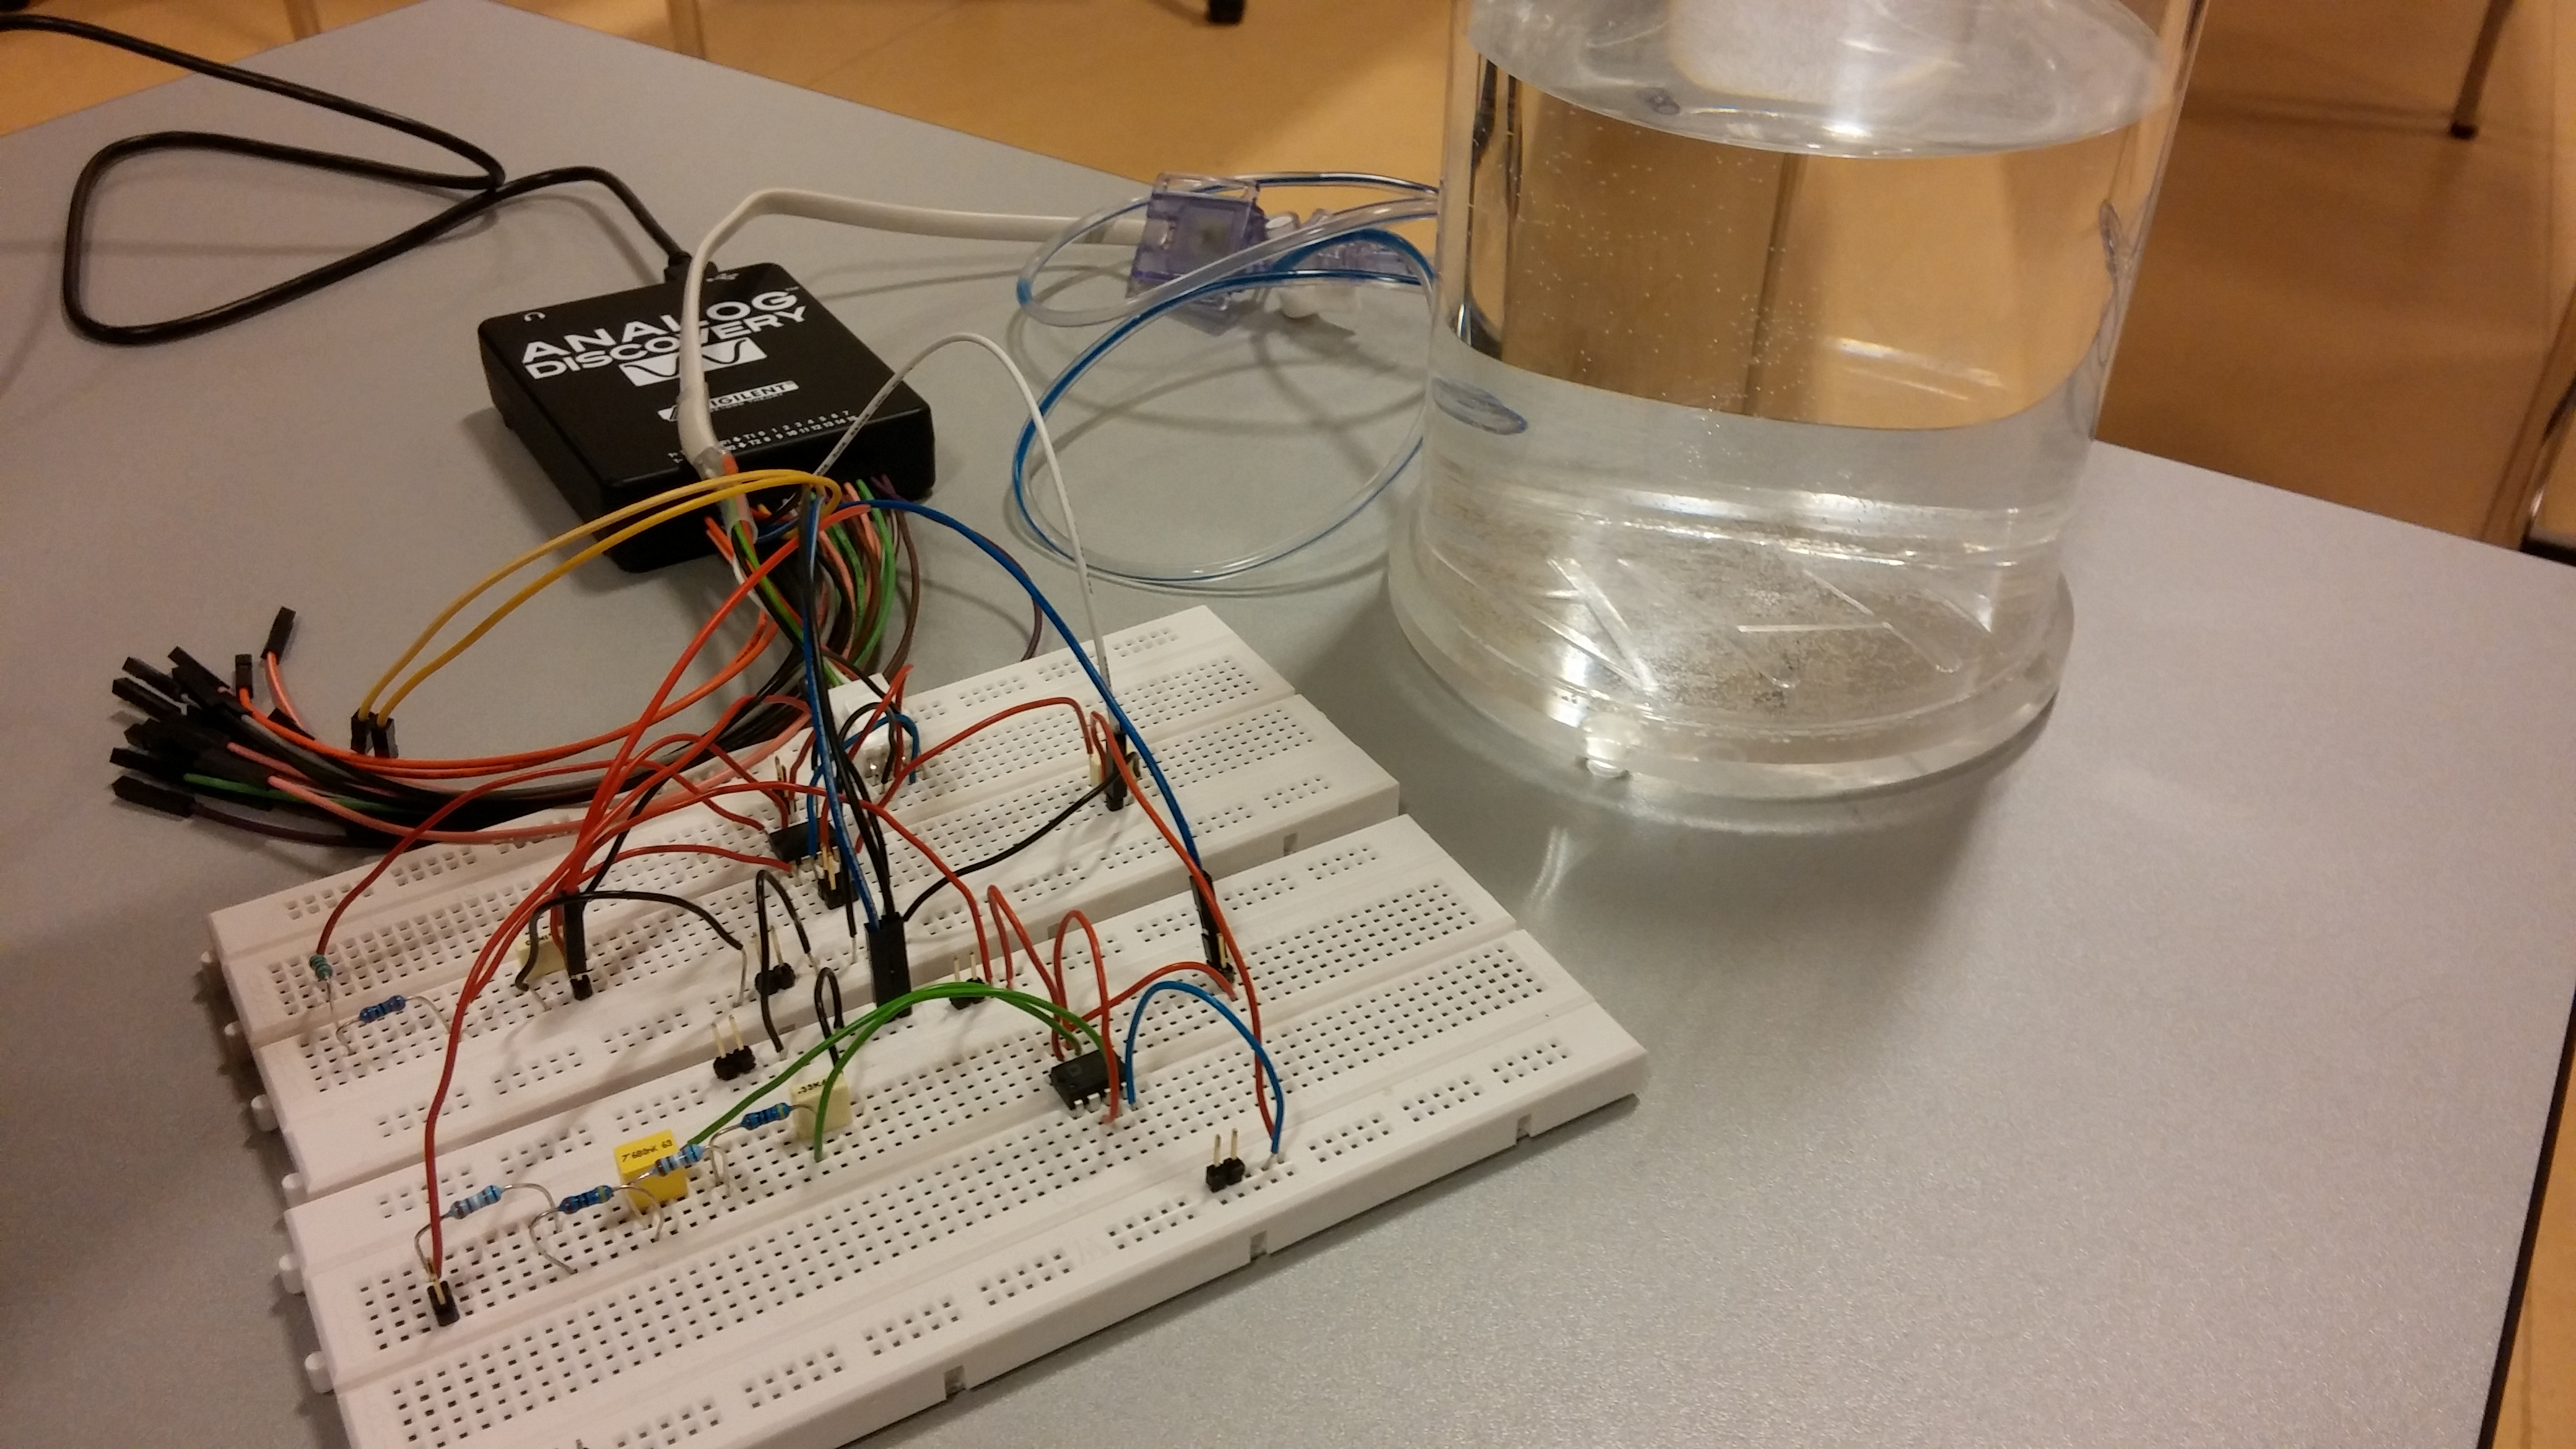
\includegraphics[width=1\textwidth]{Figurer/Hardware/IntegrationVandsoejle}
	\caption{Opstillingen som blev brugt til integrationstest af hardwaredelen med vandsøjle}
	\label{fig:IntegrationVandsoejle}
\end{figure}

Ved det kendte vandsøjletryk i mmHg blev udgangsspændingen for det analoge filter noteret i bilag \ref{Modul og integration}. Efter at have lavet lineær regression over de fem målepunkter blev tendenslinjens ligning sammenlignet med en tendenslinje, der var lavet på baggrund af fem teoretisk beregnede punkter. 

\begin{figure}[H]
	\centering
	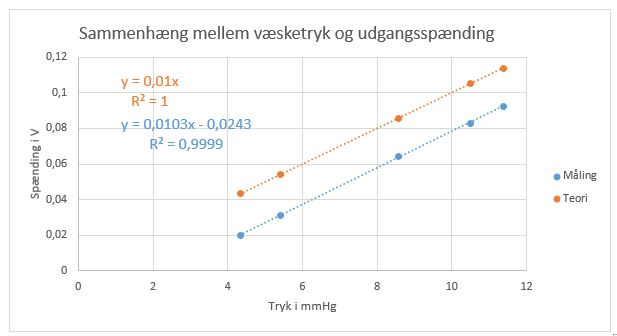
\includegraphics[width=1\textwidth]{Figurer/Hardware/VaesketrykUdgangsspaending}
	\caption{Sammenhængen mellem væsketryk input på indgangen af forstærkeren og udgangsspændingen på filteret. Angivet ved henholdsvis teoretisk beregnet punkter og målte punkter.}
	\label{fig:Vaesketryk}
\end{figure}

Ud af figur \ref{fig:Vaesketryk} ses det, at de to tendenslinjer ligger næsten parallelt. Faktisk er den målte hældningskoefficient kun 0,0003 større, end det er tilfældet for den teoretisk beregnede linje. Dvs. at de to linjer næsten er parallelle. Hvis de to linjer havde været fuldkommen parallelle, ville man med sikkerhed kunne sige, hvor stort væsketryk, der er i søjlen på baggrund af det spændingsoutput der er på udgangen af det analoge filter. I systemets tilfælde afviger hældningskoefficienten med 3\% hvilket må siges at være acceptabelt grundet måleusikkerheder.

\section{Modultest software}
Til test af softwaren er der først og fremmest foretaget modultest af  kodeelementer for at teste, om de fungerer efter hensigten. Dette er gjort ved hjælp af debug-funktionen i Visual Studio. Disse tests er foretaget løbende i udviklingsprocessen, hver gang en metode er tilføjet eller ændret. De væsenligste dele er nedenfor beskrevet: \\[1ex]
Login-funktionen er den første funktion, der er testet ved at sammenligne tilladte brugernavne og kodeord i databasen med det indtastede. Dvs. at kun de brugernavn- og kodeordssammensætninger der findes i databasen, giver adgang til systemet.\\[1ex]
Nulpunktsjusteringen er testet ved at påtrykke systemet en DC-spænding på 2V, hvorefter det indlæste tryk aflæses og sammenlignes med de 2V. \\
I forbindelse med test af nulpunktjusteringen, hvor der påsættes 2V DC-spænding, er kalibreringen også testet ved at indtaste kalibreringsfaktoren på 2. Herefter er tjekkes at signalet er forstærket 2 gange.\\[1ex]
Testene foretaget i forbindelse med indlæsning af blodtrykssignal og detektering af systole, diastole og puls er alle foretaget ved følgende:\\
Der indsættes et kendt blodtrykssignal, med kendt antal toppe og dermed kendt systole, diastole og puls. De kendte værdier sammenlignes med værdierne der vises grafisk, samt med værdierne der findes ved debugging af systemet.\\[1ex]
Alarmen er tjekket ved at påsætte et blodtrykssignal med kendte blodtryksværdier: systolisk > 160 eller < 100 og diastolisk > 100 eller < 40, hvorefter det er testet om alarmen lyder ved de fire tilfælde, uafhængigt af hinanden.\\ Yderligere for alarmen er der justering af grænseværdierne testet, ved at ændre disse grænseværdier således ovenstående værdier ikke er kritiske, for herefter at tjekke om alarmen lyder.\\ Ved alarm, er det testet at lyden kan udskydes med 3 minutter, som skrevet i koden, ved at lade blodtrykssignalet overskride grænseværdierne i mere end 3 minutter.\\[1ex]
Gemme-funktionen er testet ved at sende et kendt blodtrykssignal igennem systemet, og tjekke om de data der gemmes i databasen stemmer overen med de kendte data. I samme forbindelse er CPR-tjekker testet ved først at indskrive et gyldigt CPR-nummer, som først tjekkes i CPR-tjekker-metoden og dernæst i databasen. Derefter er samme procedure gentaget med et ikke-gyldigt CPR-nummer.


\section{Integrationstest software}
I dette afsnit vil der beskrives, hvordan systemets dele er blevet testet sammen. Dette fører videre fra modultesten, hvor de enkelte delelementer blev testet og nu vil disse delelementer blive testet sammen som et helt system. \\
For at teste det samlede software-system er der blevet lavet en integrationstest. Ved udførelsen af integrationstesten, genereres der en kendt spænding vha. Analog Discovery, der bliver sendt igennem systemet og herefter bruges debug-funktionen i Visual Studio til at se om værdierne, der bliver indlæst af systemet, stemmer overens med signalet, der sendes ind.\\
I denne test sendes der et signal igennem systemet på 4V. Det vil hermed sige, at værdierne, der indlæses burde, hvis systemet virker efter hensigten, ligge tæt på 4.
\begin{figure}[H]
	\centering
	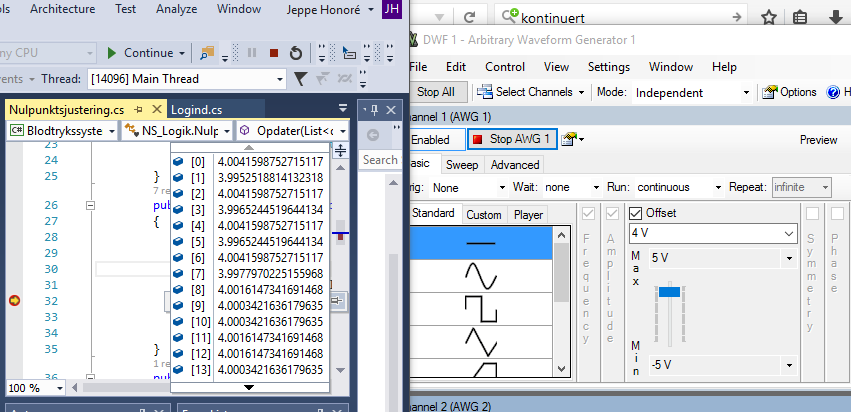
\includegraphics[width=1\textwidth]{Figurer/Softwareimplementering/Integrationstest}
	\caption{Integrationstest software}
	\label{fig:integrationstestsoftware}
\end{figure}
På figur \ref{fig:integrationstestsoftware} ses det, at de indlæste værdier ligger lige omkring 4. Det vil sige, at systemet indlæser værdierne efter hensigten.   

\section{Integrationstest system}
I dette afsnit beskrives, hvordan software-systemet testes sammen med hardware-systemet. Denne test forudsætter, at der er lavet integrationstest for både hardware og software hver for sig. \\
Denne integrationstest lægger op til accepttesten, som udføres med kunden. Det er derfor vigtigt at få de to systemer testet sammen, inden den endelige accepttest foretages. \\
\\
Transduceren kobles til vandsøjlen, hvor højden fyldes til 9cm, dvs. et tryk på 6,61mmHg, se udregning i bilag \ref{Modul og integration}. Transduceren kobles til hardwaren, og der måles på udgangene fra filtret vha. Analog Discovery. Udgangssignalet fra filtret sendes igennem DAQ’en og ind i computeren. Der sættes breakpoints i programmet ved værdien for nulpunktsjustering og værdien af signalet. 
Transduceren sættes til at måle atmosfærisk tryk, og der foretages en nulpunktsjustering i programmet. Værdien på Analog Discovery sammenlignes med værdien, der ses ved debugging i koden. Af figur \ref{fig:Atmosfaerisktryk} ses, at der kun er en forskel på 2,1mV, hvilket kan skyldes, at signalet svinger lidt, da trykket ikke er helt jævnt.

\begin{figure}[H]
	\centering
	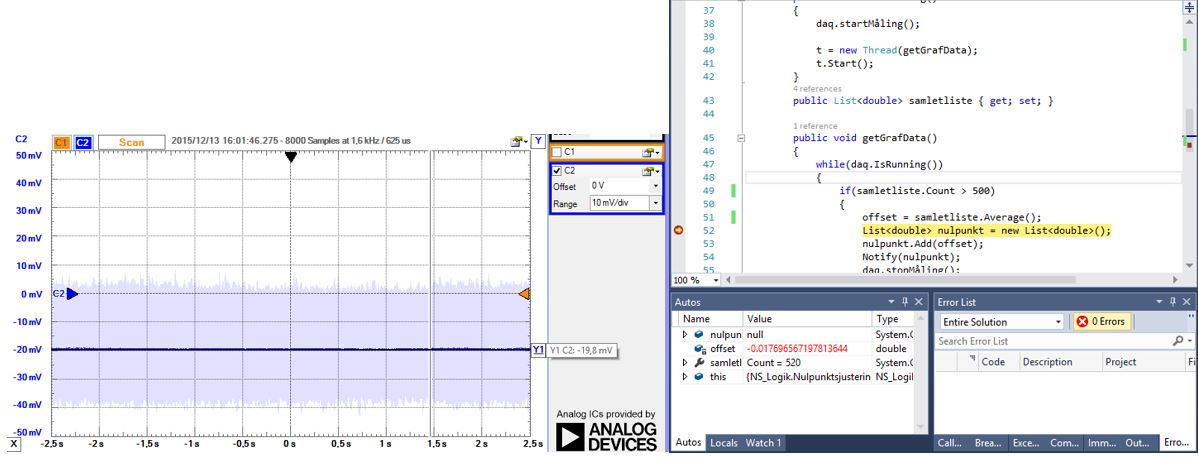
\includegraphics[width=1.2\textwidth]{Figurer/Test/Nulpunkt}
	\caption{Værdien fra det atmosfæriske tryk målt med Analog Discovery til -19,8mV (til venstre) og med programmet til -0,0177V (til højre).}
	\label{fig:Atmosfaerisktryk}
\end{figure}

Transduceren sættes til at måle trykket fra vandsøjlen. Dernæst foretages en måling i programmet. I selve koden findes værdien, der måles og denne sammenlignes med målingen i Analog Discovery. Af figur \ref{fig:Vaesketryk2} ses, at signalet, som programmet opfanger, svinger omkring værdien vi måler med Analog Discovery. Dette kan skyldes, at vandsøjlens overflade står og vibrerer med rystelserne i bordet, hvorved der skabes støj i signalet.

\begin{figure}[H]
	\centering
	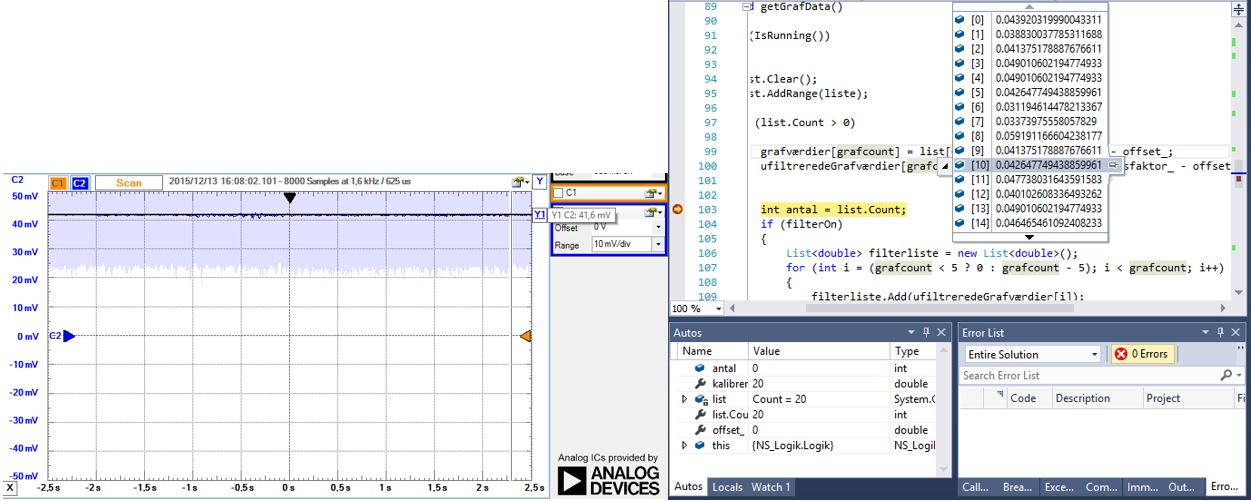
\includegraphics[width=1.1\textwidth]{Figurer/Test/Vandsoejle}
	\caption{Værdien fra væsketrykket målt med Analog Discovery til 41,6mV (til venstre) og med programmet i V (til højre).}
	\label{fig:Vaesketryk2}
\end{figure}

Dernæst sammenlignes det kendte tryk med værdien, der vises i programmet. Her ses af figur \ref{fig:mmHgtryk}, at værdien af mmHg i programmet ligger lidt under det tryk, der forventes i vandsøjlen. Dette kan skyldes måleusikkerheder fra målingen af vandsøjlens højde og ændringen af signalet undervejs i hardwaren og DAQ’en. Svingningerne af værdien i signalet skyldes stadig, at vandsøjlens overflade vibrerer når der er små vibrationer i bordet vandsøjlen står på.  

\begin{figure}[H]
	\centering
	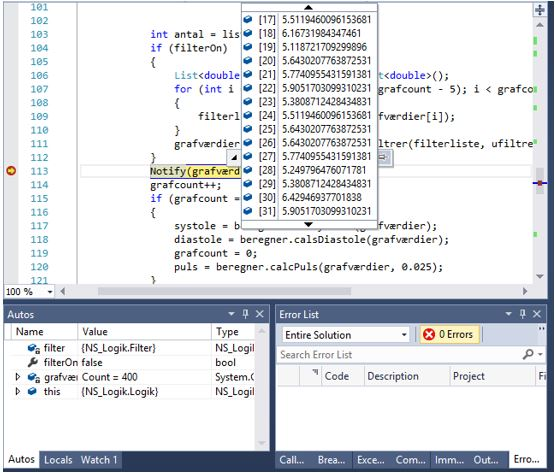
\includegraphics[width=0.6\textwidth]{Figurer/Test/mmHg}
	\caption{Værdien fra Væsketrykket målt med programmet i mmHg.}
	\label{fig:mmHgtryk}
\end{figure}